Ainda falando sobre exploração espacial, o \textit{Gateway} lunar será a primeira estação espacial a orbitar a Lua.

\subsection{Gateway lunar}

O \textit{Gateway}, conforme explica \citep{nasa_gateway}, está sendo desenvolvido pela NASA em colaboração com parceiros internacionais, incluindo a Agência Espacial Europeia (ESA), a Japan Aerospace Exploration Agency (JAXA) e a Canadian Space Agency (CSA). Essa estação espacial foi projetada para servir como um centro de comunicações movido a energia solar, e é um laboratório científico e módulo habitacional de curto prazo. O \textit{Gateway} desempenhará um papel importante no programa Artemis, que facilitará a exploração lunar e servindo como ponto de partida para futuras missões tripuladas a Marte.

Inicialmente, as primeiras estruturas serão o Elemento de Potência e Propulsão (PPE) e o Módulo de Habitação e Logística (HALO), sendo que o PPE fornecerá energia elétrica e a capacidade de propulsão, enquanto que o HALO oferecerá espaço habitável para a tripulação e interfaces para integração de outras espaçonaves. Ambos os módulos estão programados para serem lançados juntos em 2027 a bordo de um foguete Falcon Heavy.

Além dos módulos descritos, o \textit{Gateway} contará com contribuições internacionais. A ESA irá contribuir com o módulo de reabastecimento e comunicações ESPRIT, e um braço robótico de 8,5 metros, denominado Canadarm3, projetado pela CSA \citep{csa_canadarm3}. Esses dispositivos ampliarão as capacidades da estação para obter operações além do projetado inicial e suporte a diversas missões científicas e de exploração.

A órbita planejada para a estação espacial é uma órbita de halo quase retilínea (NRHO) ao redor da Lua, que permitirá um acesso facilitado à superfície lunar e servirá como um ponto estratégico para missões no espaço profundo. De acordo com \citep{esa_lunar_gateway_2019}, a altitude de perigeu (altitude mais próxima da Lua) será de 3.000km e a altitude de apogeu (altitude mais distante da Lua) será de 70.000km, essa posição orbital irá ajudar a melhorar comunicação com a Terra e proporcionará uma plataforma estável para operações científicas diversas e de exploração.

\begin{figure}[H]
    \centering
    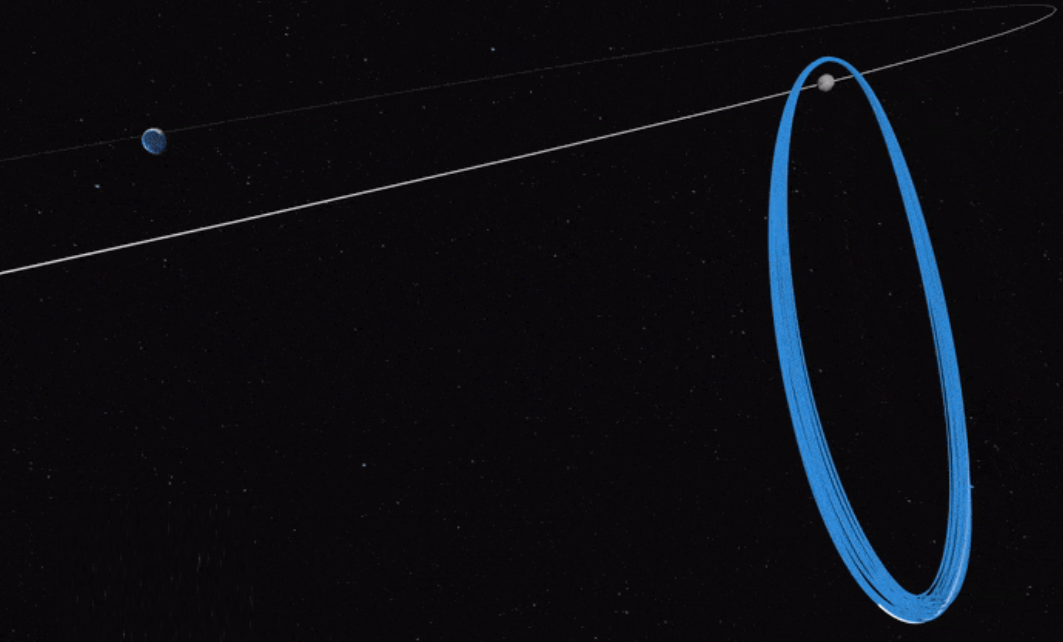
\includegraphics[width=0.75\linewidth]{Imagens/Gateway lunar NRHO orbit.png}
    \caption{Demonstração gráfica da órbita do Gateway na Lua. Fonte: ESA (\url{https://www.esa.int/ESA_Multimedia/Images/2019/07/Orbiting_lunar_Gateway}).}
    \label{fig:orbitaGatewayNRHO}
\end{figure}

Para que toda a missão do \textit{Gateway} seja viável, é importante salientar que os procedimentos de rendezvous e docking entre os veículos espaciais e a estação em órbita lunar, sem esse tipo de operação, a exploração futura não é possível, pois esses processos consistem na aproximação controlada e segura, posteriormente o acoplamento de uma espaçonave a outra estrutura orbital, exigindo coordenação entre sistemas de navegação, propulsão e controle de atitude. No contexto do \textit{Gateway}, essas manobras permitirão a chegada de tripulações, cargas, módulos adicionais e outros equipamentos desejados, além de que irá viabilizar o retorno dos veículos espaciais à Terra. A operação em órbita de halo apresenta desafios adicionais em relação à dinâmica orbital e ao planejamento de trajetórias, demandando soluções específicas, como as de rendezvous and docking, para garantir o cumprimento da missão.

